\documentclass[a4paper,11pt]{article}
\usepackage{fullpage}
\usepackage[latin1]{inputenc}
\usepackage[T1]{fontenc}
\usepackage[normalem]{ulem}
\usepackage[english]{babel}
\usepackage{listings,babel}
\usepackage{palatino}
\lstset{breaklines=true,basicstyle=\ttfamily}
\usepackage{graphicx}
\usepackage{moreverb}
\usepackage{url}
\usepackage{tweaklist}
\renewcommand{\itemhook}{\setlength{\topsep}{0pt}\setlength{\itemsep}{0pt}}
\renewcommand{\enumhook}{\setlength{\topsep}{0pt}\setlength{\itemsep}{0pt}}

\title{Time to Digital Converter Core for Spartan-6 FPGAs}
\author{S\'ebastien Bourdeauducq}
\date{November 2011}
\begin{document}
\setlength{\parindent}{0pt}
\setlength{\parskip}{5pt}
\maketitle{}
\section{Specifications}
The Time to Digital Converter (TDC) core is a high precision (sub-nanosecond) time to digital conversion core for Xilinx Spartan-6 FPGAs.

\begin{itemize}
\item Expected precision: 50-100ps (peak to peak).
\item Fixed point output:
\begin{itemize}
\item Integer part is number of FPGA clocks (coarse counter).
\item 13-bit fractional part (configurable with a VHDL generic).
\item With a 125MHz FPGA clock, LSB corresponds to 0.98ps.
\end{itemize}
\item Typical range: 268ms (using a <25.13>-bit value at 125MHz).
\begin{itemize}
\item Number of coarse counter bits configurable with a VHDL generic.
\end{itemize}
\item Latency: 6 cycles at 125MHz (not including host interface module).
\item Multiple channels.
\begin{itemize}
\item Configurable with a VHDL generic.
\item Calibration logic shared between channels.
\end{itemize}
\item Reports both rising and falling edges of the input signal.
\item Input signal must not have transitions shorter than three times the FPGA clock period (e.g.\ the frequency of the input signal must be less than one sixth of the FPGA clock).
\item Uses a counter for coarse timing and a calibrated delay line for fine timing.
\item Delay line implemented with carry chain (\verb!CARRY4!) primitives.
\item Calibration mechanism:
\begin{itemize}
\item at startup (and after receiving a reset command), send random pulses into the delay line (coming from e.g. a on-chip ring oscillator), build histogram, compute delays (as explained in the Fermilab paper \cite{fermilab}, initialize the LUT, and measure the frequency of the compensation ring oscillator.
\item for online temperature/voltage compensation, measure again the frequency of the ring oscillator, compare it to the frequency measured at start-up, linearly interpolate the delays, and update the LUT.
\end{itemize}
\item "Wave union" not implemented.
\item Input signals (without host interface module):
\begin{itemize}
\item Input signal.
\item Calibration signal.
\item Coarse counter reset.
\item Per-channel de-skew value.
\item Full reset (and recalibrate).
\item Clock.
\end{itemize}
\item Output signals (without host interface module):
\begin{itemize}
\item Startup calibration in progress.
\item Periodic counter overflow.
\item Received rising/falling edge notification:
\begin{itemize}
\item Strobe signal.
\item Rising/falling edge.
\item Fixed point timestamp.
\item Raw encoded value from the delay line.
\end{itemize}
\end{itemize}
\item Debug interface:
\begin{itemize}
\item Forced switch to the calibration signal.
\item Access to the histogram values from the startup calibration.
\item Access to the frequencies of the online calibration ring oscillators.
\end{itemize}
\item Optional host/CPU interface module:
\begin{itemize}
\item Wishbone slave.
\item Configuration and status registers.
\item Interrupts: edge received, counter overflow.
\end{itemize}
\end{itemize}

\section{Architecture}
\subsection{Overview}
The block diagram of the core is given in Figure~\ref{fig:block}.

\begin{figure}[h]
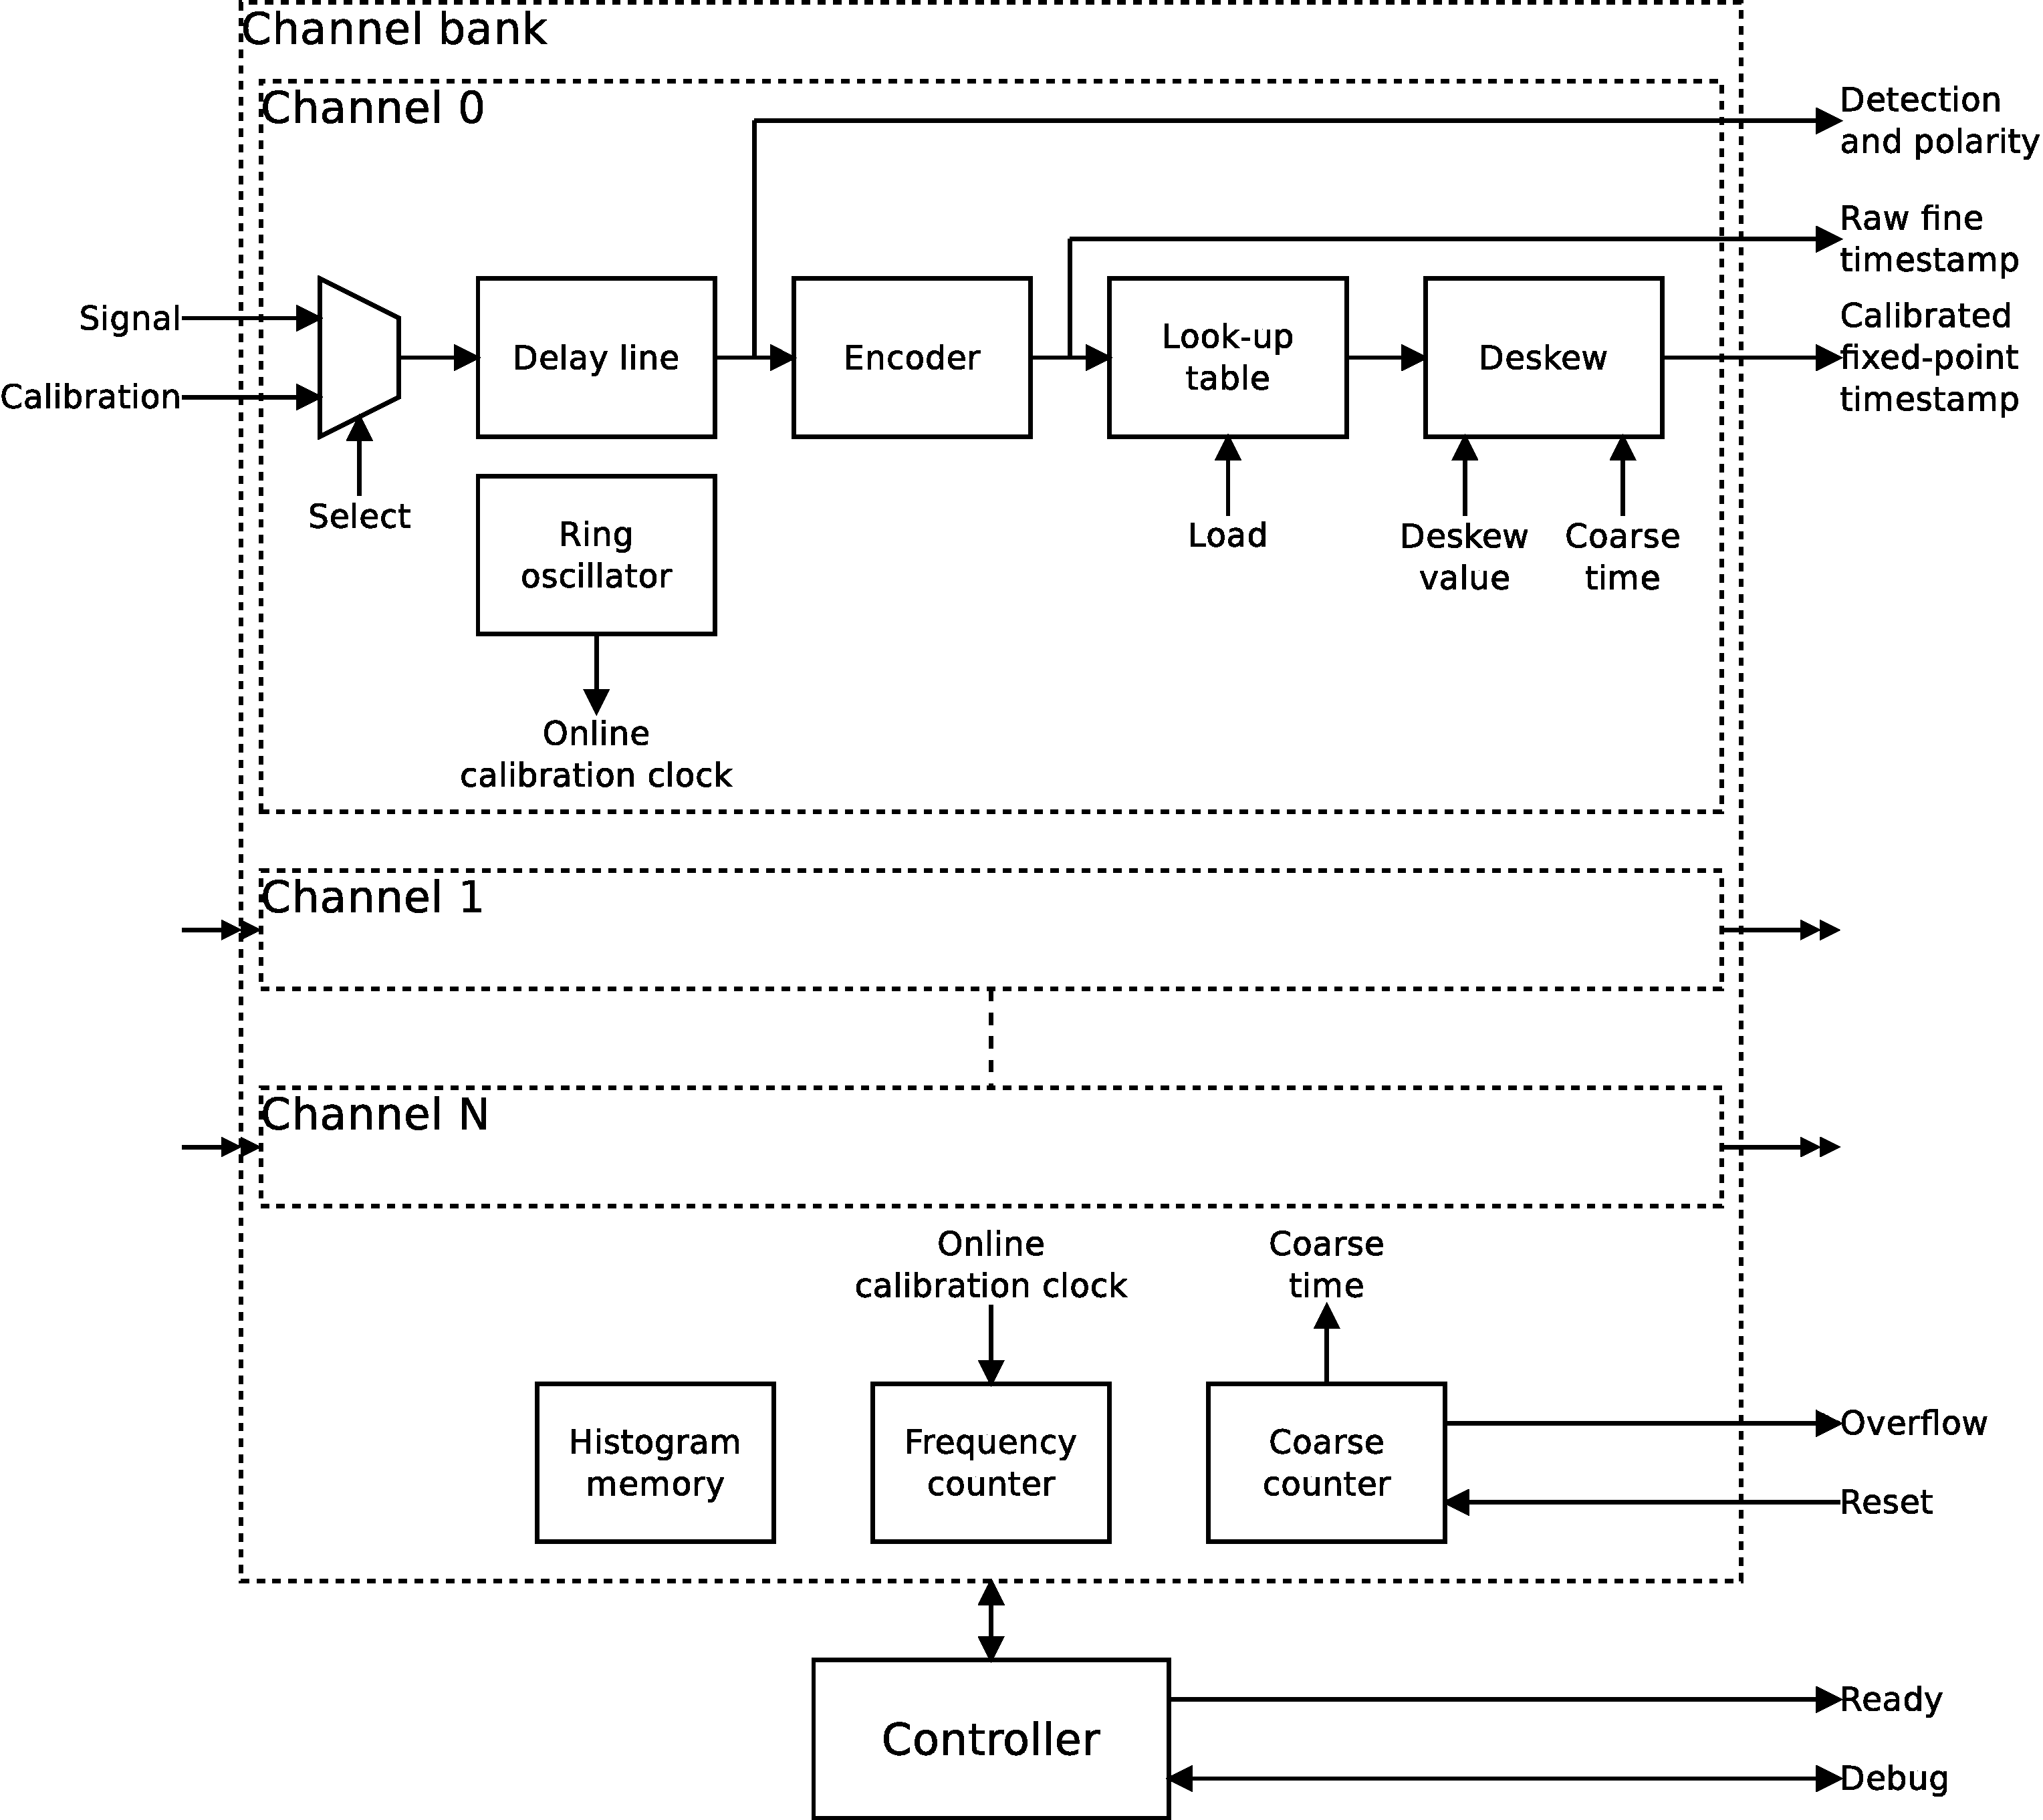
\includegraphics[width=\textwidth]{block.pdf}
\caption{Block diagram of the TDC core.}
\label{fig:block}
\end{figure}

The signal to be timestamped is injected into a tapped delay line to obtain a fine time measurement (below the clock period). The total delay of the delay line must be greater than the clock period. At each clock tick, an encoder counts the taps the signal has reached and gives a \textit{raw} measurement of the timestamp of the signal within the current clock cycle. This raw value is fed into a look-up table (LUT) which converts it into a calibrated value expressed in subdivisions of the clock cycle, called the \textit{fractional} value. Finally, in the \textit{deskew} stage, the fractional value is combined with the index of the current clock cycle given by the coarse counter, and the resulting fixed-point value is added a user-defined constant to enable the TDC core to directly generate timestamps relative to the source of the system clock.

The main difficulty with this system is that the delay line is subject to process, temperature and voltage (PVT) induced variations, and it needs to be calibrated against them.

To generate the LUT contents, the controller switches to the calibration signal. The key property of the calibration signal is that the probability density of its transition timestamps within a system clock cycle must be constant. The controller measures the raw timestamps and books a histogram. Because of the constant probability density, the heights of the histogram bars are approximately proportional to the delays between the taps of the delay line after enough measurements have been taken. Further, the last tap to have recorded a signal transition corresponds to a delay equal to the system clock period. This enables the controller to build the initial contents of the LUT. This process is called \textit{startup calibration}.

The drawback of the startup calibration is that the system cannot operate while the calibration is taking place. Therefore, a process of \textit{online calibration} has been devised. Each channel contains a ring oscillator that is placed close to the delay line. The controller periodically measures the frequency of this ring oscillator, compares it to the frequency that was measured at the time of startup calibration, linearly interpolates the fractional timestamps, and updates the LUT. This allows compensation of temperature and voltage effects while the system keeps running.

The system gives timestamps of both rising and falling edges of the incoming signal. The rising edges are discerned from the falling edges using the ``polarity'' output.

\subsection{Delay line structure}
\label{delaystruct}
The delay line uses a carry chain. It is made up of \verb!CARRY4! primitives whose \verb!CO! outputs are registered by the dedicated D flip flops of the same slices. The signal is injected at the \verb!CYINIT! pin at the bottom of the carry chain. The \verb!CARRY4! primitives have their \verb!S! inputs hardwired to 1, which means the carry chain becomes a delay line with the signal going unchanged through the \verb!MUXCY! elements (see \cite{s6hdl} for reference). Since each \verb!CARRY4! contains four \verb!MUXCY! elements, the delay line has four times as many taps as there are \verb!CARRY4! primitives.

Using the Xilinx timing model, a surprising observation is that some delay differences between consecutive taps are negative. This probably is at the origin of the ``bubbles'' mentioned in the EPFL paper \cite{epfl}. The schematics given by Xilinx of the \verb!CARRY4! primitive is misleading there, and has probably little to do with the actual transistor-level implementation. The Xilinx documentation \cite{s6hdl} gives a hint by describing the primitive as ``Fast Carry Logic \textit{with Look Ahead}''.

To avoid negative differences, we simply reorder the bits at the output of the delay line to sort the taps by increasing actual delays. We can then think of the delay line according to Figure~\ref{fig:delaystruct}. The bin widths are uneven, but the incoming signal reaches the taps in order. This last property simplifies the encoder design, since it only has to count the number of identical bits at the beginning of the delay line.

\begin{figure}[h]
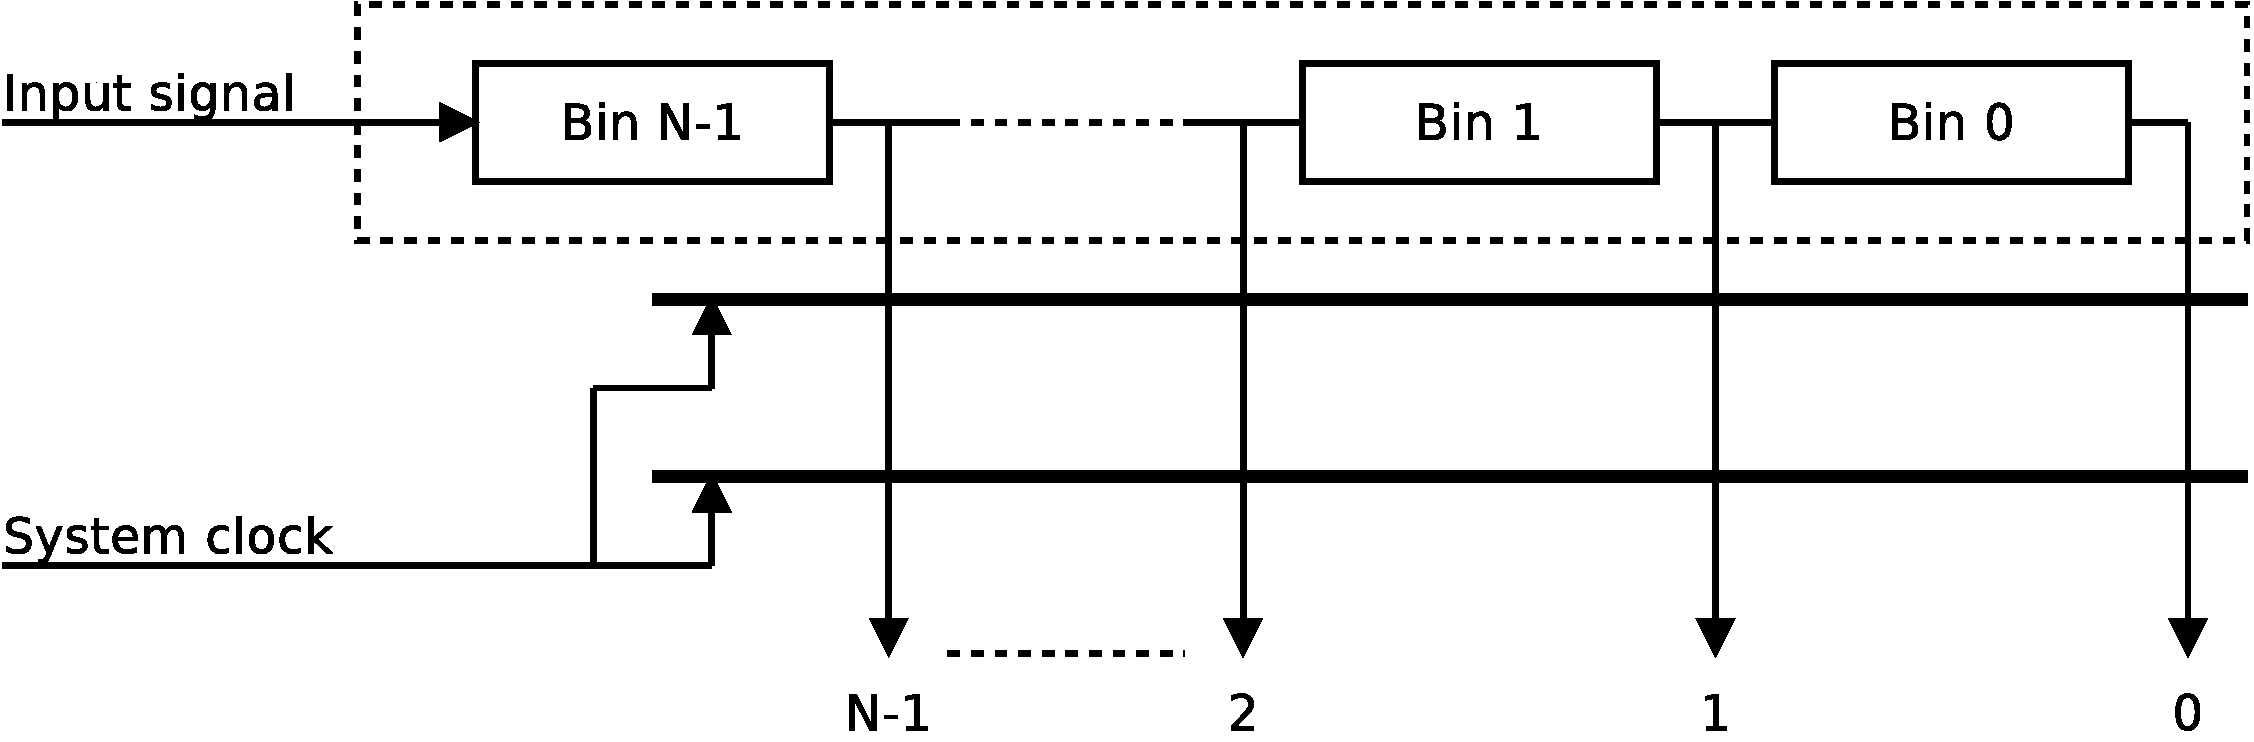
\includegraphics[width=\textwidth]{delaystruct.pdf}
\caption{Representation of the delay line.}
\label{fig:delaystruct}
\end{figure}

\subsection{Calibration details}
In the formulas below:
\begin{itemize}
\item $T_{sys}$ is the system clock period.
\item $H(n)$ is the number of hits in the histogram at output $n$. A hit at output $n$ means that the signal propagated down to output $n$, without reaching output $n-1$.
\item $W(n)$ is the width of bin $n$.
\item $C = \displaystyle\sum\limits_{n=0}^{N-1} H(n)$ is the total number of hits in the histogram.
\item $R(n)$ is the timestamp of an event whose signal propagated down to output $n$ (without reaching output $n-1$), measured backwards from the clock tick.
\item $f$ (respectively $f_{0}$) is the current (respectively reference) frequency of the online calibration ring oscillator.
\end{itemize}

\subsubsection{Offline calibration}
We take the first output of the delay line to be the origin of the time measurements, and we define:
\begin{equation}
W_{0}(N-1) = 0
\end{equation}

The width of other bins is proportional to their respective number of counts in the histogram. The widths sum up to a clock period. This leads to the following equation:
\begin{equation}
W_{0}(n) = \frac{H(n+1)}{C} \cdot T_{sys}
\end{equation}

The timestamp is the sum of the widths of the traversed bins:
\begin{equation}
R_{0}(n) = \displaystyle\sum\limits_{i=n}^{N-1}{W_{0}(i)} = \frac{T_{sys}}{C} \cdot \displaystyle\sum\limits_{i=n}^{N-1}{H(i)}
\end{equation}

In the TDC core, the unit is the clock period, and the output has $F$ base 2 digits after the radix points. The controller also chooses $C=2^{F+P}$, where $P$ is the number of \textit{extra histogram bits}. Expressed in units of $2^{-F}$ clock periods (which is the weight of the least significant bit of the fixed-point output), we have:
\begin{equation}
\frac{T_{sys}}{C}=2^{-P}
\end{equation}

\subsubsection{Online calibration}
Online calibration is performed with a simple linear interpolation of the delays relative to the ring oscillator frequencies:
\begin{equation}
R(n) = \frac{f_{0}}{f} \cdot R_{0}(n)
\end{equation}

Note that when $f < f_{0}$, some values can go above the maximum fractional part value of $1 - 2^{-F}$ and might not fit in the LUT anymore. However, those correspond to delays that now exceed one clock period, and therefore they should almost never get used. In case of overflow, the controller saturates the result by using the maximum value $1 - 2^{-F}$ in order to give the best approximation in case those LUT entries still get used.

\section{Implementing the core}
\subsection{Generics}
\label{topgenerics}
The top-level entity \verb!tdc! has the following generics:
\begin{itemize}
\item \verb!g_CHANNEL_COUNT! is the number of channels supported by the core. It can be arbitrarily large. However, because the control logic is shared, adding more channels increases the startup calibration time and the delay between two consecutive online calibrations of any given channel.
\item \verb!g_CARRY4_COUNT! is the number of \verb!CARRY4! elements in the delay line of each channel. Each \verb!CARRY4! has 4 outputs, so the number of taps of the delay line is $4 \cdot \verb!g_CARRY4_COUNT!$.
\item \verb!g_RAW_COUNT! represents the number of bits at the output of the encoder. It should be set to the smallest value that verifies $4\cdot \verb!g_CARRY4_COUNT! \le 2^{\verb!g_RAW_COUNT!}-1$.
\item \verb!g_FP_COUNT! defines the number of desired digits after the radix point.
\item \verb!g_EXHIS_COUNT! defines the number of desired extra histogram bits. Extra histogram bits improve precision by increasing $C$ and averaging statistical errors out.
\item \verb!g_COARSE_COUNT! is the size, in bits, of the coarse counter which is incremented at each cycle.
\item \verb!g_RO_LENGTH! defines how many \verb!LUT! primitives used as inverters are chained in the ring oscillator of each channel. For the ring oscillators to operate, this number must be odd.
\item \verb!g_FCOUNTER_WIDTH! is the width, in bits, of the counter used to measure the frequency of the ring oscillator. Increasing this width allows for a more precise frequency measurement.
\item \verb!g_FTIMER_WIDTH! defines the duration during which the frequency counter will count the rising edges of the ring oscillator signal. This duration is approximately equal to $2^{\verb!g_FTIMER_WIDTH!}$ system clock cycles. The duration should be small enough so that the counter (whose size is \verb!g_FCOUNTER_WIDTH! bits) will never overflow. It should be large enough so that the maximum ``dynamic range'' of the counter is used.
\end{itemize}

\subsection{Ports}
The top-level entity has the following ports. All signals are synchronous to the system clock and active high.
\begin{itemize}
\item \verb!clk_i! is the system clock.
\item \verb!reset_i! is the active high synchronous global reset. The core performs startup calibration after this signal has been asserted.
\item \verb!ready_o! is held high after the startup calibration is complete.
\item \verb!cc_rst_i! resets the coarse counter.
\item \verb!cc_cy_o! is pulsed when the coarse counter overflow. In other words, it is the coarse counter carry output.
\item \verb!deskew_i! defines the per-channel deskew values added to all measurements. Each channel uses \verb!g_COARSE_COUNT!+\verb!g_FP_COUNT! bits. The value can be negative, using two's complement representation.
\item \verb!signal_i! is the per-channel signal input (one bit per channel).
\item \verb!calib_i! is the per-channel calibration signal input (one bit per channel). The calibration signal should not have transitions shorter than \textbf{three} periods of the system clock. If an oscillator is used to generate this signal, its frequency must be set to less than \textbf{one sixth} of the system clock.
\item \verb!detect_o! is pulsed after a transition of the input signal (one bit per channel). This signal should be ignored when \verb!ready_o! is low.
\item \verb!polarity_o! indicates the detected edge type. If the value is 1, it means the core has detected a rising edge. If it is 0, it means a falling edge. There is one bit per channel.
\item \verb!raw_o! gives the raw encoded timestamp, i.e.\ the number of reached taps in the delay line. There are \verb!g_RAW_COUNT! bits per channel.
\item \verb!fp_o! is the fixed-point calibrated timestamp. There are \verb!g_COARSE_COUNT!+\verb!g_FP_COUNT! bits for each channel.
\end{itemize}

The signals \verb!deskew_i!, \verb!signal_i!, \verb!calib_i!, \verb!polarity_o!, \verb!raw_o! and \verb!fp_o! correspond to multiple channels. The vectors of each channel are simply concatenated to form one larger vector, with the first channel taking the least significant bits, the second channel taking the next bits, and so forth. For example, if \verb!g_RAW_COUNT! is 10 and \verb!g_CHANNEL_COUNT! is 3, channel 0 will use bits 0 to 9 of \verb!raw_o!, channel 1 will use bits 10 to 19, and channel 2 will use bits 20 to 29.

For each channel, the signals \verb!polarity_o!, \verb!raw_o! and \verb!fp_o! are strobed by the \verb!detect_o! signal. Additionally, they remain constant until the next assertion of \verb!detect_o!.

\subsection{Debug ports}
The debug interface allows external access to LUT contents, histogram contents, and frequency counter. If it is not desired, connect \verb!freeze_req_i! to 0. The other signals then become ``don't-care''.

To enable the debug interface, assert \verb!freeze_req_i! and keep it asserted. The controller will stop performing online calibration and give you access to the channel bank controls. When the controller has given you access, it asserts the \verb!freeze_ack_o! signal. To re-enable the controller and resume the online calibration cycles, simply deassert \verb!freeze_req_i!.

The debug interface operates on a single channel at once. The channels are selected in turn using the \verb!cs_next_i! and \verb!cs_last_o! signals.

All signals are synchronous to the system clock and active high.
\begin{itemize}
\item \verb!freeze_req_i! requests control of the channel bank and activation of the debug interface.
\item \verb!freeze_ack_o! acknowledges activation of the debug interface.
\item \verb!cs_next_i! is pulsed to switch to the next channel. If \verb!cs_last_o! is active, it switches to the first channel.
\item \verb!cs_last_o! indicates that the debug interface currently operates on the last channel.
\item \verb!calib_sel_i! switches the input of the current channel to the calibration signal.
\item \verb!lut_a_i! selects an address to read in the current channel's LUT.
\item \verb!lut_d_o! returns the read LUT data one cycle of latency after a valid \verb!lut_a_i! signal.
\item \verb!his_a_i! selects an address to read in the current channel's histogram.
\item \verb!his_d_o! returns the read histogram data one cycle of latency after a valid \verb!his_a_i! signal.
\item \verb!oc_start_i! is pulsed to start a ring oscillator frequency measurement in the current channel.
\item \verb!oc_ready_o! is asserted when the frequency counter is not currently performing a measurement.
\item \verb!oc_freq_o! returns the measured ring oscillator frequency. It is valid only when \verb!oc_ready_o! is asserted.
\item \verb!oc_sfreq_o! returns the ring oscillator frequency of the current channel that was stored during startup calibration.
\end{itemize}

\subsection{Synthesis and physical implementation notes}
\subsubsection{Retiming}
The encoder design relies on the synthesis tool to push its two pipelining registers into the processing logic. The VHDL code sets the Xst-specific \verb!register_balancing! property on the registered signals for this optimization to happen. Make sure that your synthesis tool honors this property (or its equivalent), or enable retiming globally in your design.

\subsubsection{Full implementation of the ring oscillator}
Even when the optimization of instantiated primitives is disabled in the Xst options, it still turns the chain of inverting \verb!LUT! primitives into a single \verb!LUT!, which renders the ring oscillator inoperative. To prevent this, the Xst-specific \verb!keep! property is set by the source code on the internal ring oscillator signals. Make sure that your synthesizer honors it.

\subsubsection{False timing paths}
The calibration selection signal is driven synchronously by the controller, and the output of the multiplexer goes through the delay line before being recaptured synchronously by the input flip-flops. The automatic place and route tool incorrectly assumes this is a regular synchronous path. Since the delay line is always longer than a clock period, it aborts with a message saying that the components delays alone exceed the timing constraints. The problem is resolved by adding ``timing ignore'' (TIG) constraints into the UCF file, using a syntax based on the example below:
\begin{verbatim}
NET "cmp_tdc/cmp_channelbank/g_single.cmp_channelbank
/cmp_channel/muxed_signal" TIG;
\end{verbatim}

Or, for multiple channels:
\begin{verbatim}
NET "cmp_tdc/cmp_channelbank/g_multi.cmp_channelbank
/g_channels[0].cmp_channel/muxed_signal" TIG;
NET "cmp_tdc/cmp_channelbank/g_multi.cmp_channelbank
/g_channels[1].cmp_channel/muxed_signal" TIG;
\end{verbatim}

One constraint must be added per channel, and the numbers ``0'', ``1'', ... incremented accordingly.

\subsubsection{Delay line placement}
The delay line must be placed in a way that minimizes the delay from the input signals IOBs. The reason is that this delay is affected by PVT variations that are not compensated for.

\subsubsection{Ring oscillator placement}
To be most effective, the ring oscillator must be placed close to the delay line of the same channel.

\subsubsection{Reordering taps}
To avoid negative delay differences (section \ref{delaystruct}), examine the timing report for the delay line and edit \verb!tdc_ordertaps.vhd! to reorder the taps by increasing delays.

The script \verb!ordertaps.py! can be used to automate this task. See the comments at the beginning of the script for details.

\section{Simulation}
\subsection{Overview}
The TDC core comes with unit tests for several of its modules. Simulations are typically performed using the free GHDL tool, but the test benches should be compatible with other VHDL simulators. To run simulations with GHDL, use the \verb!simulate.sh! script in each test bench's folder.

\subsection{Encoder test -- lbc}
This test verifies the pipelined encoder by presenting a new test vector with an alternating polarity at each clock cycle.

The encoder should count the number of leading bits of the input that have a value opposite to the polarity of the previous vector, until it reaches the first bit with a different value. It should ignore the subsequent bits. The polarity of a vector is the value of its most significant bit (and it defines whether a leading or a falling edge is being detected by the TDC core).

To validate this behaviour, the test bench generates multiple vectors of $2^{\verb!g_N!}-1$ bits each, built by concatenating $i$ bits of the current polarity, one bit with the opposite polarity (except for the last vector), and $2^{\verb!g_N!}-i-2$ random bits, for all $1 \le i < 2^{\verb!g_N!}$. The polarity alternates at each cycle, which means the encoder should always detect a new event.

The test bench verifies that the encoder produces the correct integer sequence $1, ..., 2^{\verb!g_N!}-1$ after its two cycles of latency, and that the polarity detection output is toggling.

The test bench is self-checking and will produce a failed assertion in case of an unexpected value.

The value \verb!g_N! is configurable with a generic.

\subsection{Frequency counter test -- freqc}
This test bench generates a system clock and a measured clock, measures the latter using the frequency counter module, and verifies the result.

It is self-checking and will produce a failed assertion in case the counter has too much inaccuracy; that is, if the measured clock cycle counter differs by more than one unit from the best possible value.

The generics of the test bench are:
\begin{itemize}
\item \verb!g_COUNTER_WIDTH!: see \verb!g_FCOUNTER_WIDTH! in subsection \ref{topgenerics}.
\item \verb!g_TIMER_WIDTH!: see \verb!g_FTIMER_WIDTH! in subsection \ref{topgenerics}.
\item \verb!g_CLK_PERIOD!: period (in nanoseconds) of the simulated system clock.
\item \verb!g_CLK_M_PERIOD!: period (in nanoseconds) of the simulated measured clock.
\end{itemize}

\subsection{Integer divider test -- divider}
This test validates the integer divider by making it compute the quotient and remainder of all $0 ... 2^{\verb!g_WIDTH!}$ positive integer values by all $1 ... 2^{\verb!g_WIDTH!}$ values.

The test bench is self-checking and will produce a failed assertion in case the divider yields an incorrect quotient or remainder value.

The value \verb!g_WIDTH! is configurable with a generic.

\subsection{Controller test -- controller}
This test verifies the correct operation of the controller in the following scenario:
\begin{enumerate}
\item The test bench resets the controller, which begins to perform startup calibration operations.
\item The test bench sends a series of pulses with incrementing fine time stamps into the controller.
\item The test bench provides a model of the histogram memory to the controller. Because of the continuously incrementing time stamps provided by the test bench, the controller books a histogram with the same $2^{\verb!g_FP_COUNT!-\verb!g_RAW_COUNT!}$ value everywhere.
\item The controller reads the frequency of the calibration ring oscillator, and the test bench returns 1.
\item The controller performs a first round of online calibration. It reads again the frequency of the ring oscillator, and the test bench returns 2. This means that all delays should be halved.
\item The controller builds the LUT. The test bench provides a model of the memory for this purpose.
\item The controller asserts the ready signal, and this terminates the simulation.
\end{enumerate}

The test bench then verifies that the LUT entries from $i = 1$ to $i = 2^{\verb!g_RAW_COUNT!}-1$ all have the correct value, and reports a failed assertion otherwise:
\begin{equation}
\textrm{LUT}(i) = \frac{1}{2}\cdot(i-1)\cdot2^{\verb!g_FP_COUNT!-\verb!g_RAW_COUNT!}
\end{equation}

The test bench has the generics \verb!g_RAW_COUNT!, \verb!g_FP_COUNT! and \verb!g_FCOUNTER_WIDTH!, which have the same meaning as in subsection \ref{topgenerics}.

The controller depends on the divider module.

\section{Host interface module}
The optional host interface module connects the TDC core to a Wishbone bus. It is a separate top-level entity named \verb!tdc_hostif! that instantiates \verb!tdc!. It implements a Wishbone slave interface, which is automatically generated with \verb!wbgen2!.

It supports a maximum of 8 channels. The debug interface of the TDC core is also exposed through the Wishbone interface. Interrupts are generated at the end of the startup calibration, on a coarse counter overflow, and after each transition of the input signals.

Generics and ports should be self-explanatory. Refer to the documentation generated by \verb!wbgen2! for a description of the registers and interrupts. Run the \verb!genwb.py! script to generate the \verb!wb! file for \verb!wbgen2!.

\begin{thebibliography}{99}
\bibitem{s6hdl} Xilinx, \textsl{Spartan-6 Libraries Guide for HDL Designs}, \url{http://www.xilinx.com/support/documentation/sw_manuals/xilinx12_3/spartan6_hdl.pdf}
\bibitem{epfl} Claudio Favi and Edoardo Charbon, \textsl{A 17ps Time-to-Digital Converter Implemented in 65nm FPGA Technology}, ACM 2009, \url{http://infoscience.epfl.ch/record/139431}
\bibitem{fermilab} Jinyuan Wu and Zonghan Shi, \textsl{The 10-ps Wave Union TDC: Improving FPGA TDC Resolution beyond Its Cell Delay}, IEEE 2008, \url{http://www-ppd.fnal.gov/EEDOffice-W/Projects/ckm/comadc/PID765918.pdf}
\end{thebibliography}

\end{document}
